\cotefile{80}
\scanpage{22}
\mspage{3}
liest Deutsch. Vielleicht könnte ich all das, was irgendwie direkt ``autobiographisch'' ist, auf Französisch schreiben -- doch eingehende Meditationen, \unsure{insbesondére|insbesondere} an Hand von deutschsprachigem Material, auf Französisch?

Die Möglichkeit fiel mir auch ein, die beiden obigen Ansätze simultan durchzuführen -- nämlich eine \unsure{Chronologische|chronologische} Untersuchung über mein Leben \inserted{sofort} anzufangen, und zu gleicher Zeit die Lektüre etwa meines Briefwechsels mit \unsure{Hanka}.

zu befürchten wär, dass ich dauernd dabei wäre, nicht vorhandene Erinnerungen zusammenzukratzen zu versuchen! Von dort aus würden \deleted{sich} sicher viele Kernfragen \deleted{\unsure{behandelt|beantworten}} \inserted{auftauchen} und \deleted{\unsure{be}} \deleted{\unsure{behandelt}} \inserted{untersucht} werden, möglicherweise auch andere Perioden \deleted{\unsure{sichtbar}} \inserted{zur} Untersuchung aufdrängen. Wenn die Untersuchung der Kernperiode oder des Ausgangsmaterials fürs erste beendet wäre, wäre die Zeit vielleicht ``reifer'', um mich an eine chronologische Folge zu halten. Jedenfalls
% archive sheet number: 21
\scanpage{23}
Cas cruciaux d'arrangements 1-dimensionnels de $N$ ps. droites, où $N\geq\deleted{\unsure{3|5}}4$ (le cas $N=3$ étant \deleted{\unsure{élémentaire}} et bien entendu)

$1^\circ)$ Cas où il existe une ps. droite bigonale.

\margin{$N\geq4$\\ $N+1$ sommets}
$\mathrm{I}_{N})$ faisceau de $\inserted{n=}N-1\inserted{\geq3}$ ps. droites \deleted{passant par un sommet} \inserted{concourantes}, et d'une ps. droite sécante (cas où la \deleted{ps. droite} bigonale est unique)
\figure{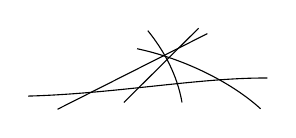
\begin{tikzpicture}[scale=.62]
\draw (0,.35) .. controls (1.8,.40) and (3.5,.73) .. (4.9,.72);
\draw (.6,.08) -- (3.67,1.63);
\draw (1.96,.22) -- (3.49,1.74);
\draw (2.45,1.69) .. controls (2.78,1.28) and (3.05,.79) .. (3.15,.22);
\draw (2.23,1.32) .. controls (3.13,1.13) and (4.12,.67) .. (4.76,.09);
\end{tikzpicture}}

\margin{$pq+2$ sommets\\ $N\geq5$}
$\mathrm{I}_{pq})$ Système formé de deux faisceaux de \inserted{$p$ et $q$} ps. droites concourantes $(p\geq q\geq2)$ plus \deleted{\unsure{leur|une}} ps. droite passant par les sommets de ces deux faisceaux $(p+q+1=N)$ (Cas de la ps. droite bigonale unique)
\figure{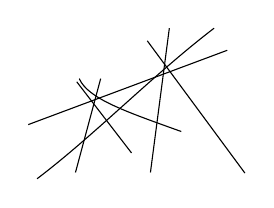
\begin{tikzpicture}[scale=.8]
\draw (.1,.92) -- (3.26,2.10);
\draw (.24,.06) .. controls (1.15,.75) and (2.07,1.70) .. (3.05,2.45);
\draw (.85,.16) -- (1.25,1.65);
\draw (.87,1.60) -- (1.74,.47);
\draw (.91,1.65) .. controls (1.05,1.33) and (1.64,1.13) .. (2.53,.81);
\draw (2.04,.16) -- (2.34,2.45);
\draw (1.99,2.25) -- (3.54,.15);
\end{tikzpicture}}

$2^\circ)$ Il n'existe pas de ps. droite bigonale \deleted{\unsure{de}}

\margin{$pq+2$ sommets\\ $N\geq5$}
$\deleted{\unsure{\mathrm I|\mathrm{II}}}\mathrm{II}_{pq})$ Système formé de deux faisceaux de $p$ et $q$ ps. droites concourantes $p\deleted{>}\geq q\geq2$, $p+q\deleted{\unsure{\geq}}=N\geq5$ (les deux faisceaux \unsure{incl.|i.e.} leurs sommets sont \deleted{\unsure{en pos}} alternés, \deleted{\unsure{le}} le cas ``minimal'' $p=\deleted{\unsure{3|2}}\unsure{2|3}$, $q=2$ est particulièrement intéressant\deleted{\unsure{)}}).
\figure{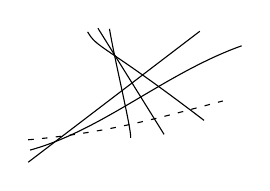
\begin{tikzpicture}[scale=.77]
\draw (0,.04) -- (2.83,2.20);
\draw (.03,.24) .. controls (1.23,.57) and (2.26,1.51) .. (3.52,1.96);
\draw[dash pattern=on 2pt off 3pt] (0,.41) .. controls (1.35,.53) and (2.14,.77) .. (3.21,1.05);
\draw (.98,2.19) .. controls (1.14,1.91) and (1.25,1.99) .. (2.90,.73);
\draw (1.15,2.25) -- (2.24,.50);
\draw (1.34,2.24) .. controls (1.43,1.70) and (1.70,.60) .. (1.69,.44);
\end{tikzpicture}}

\margin{$6$ sommets}
$\mathrm{II}_{4})$ \deleted{4 ps. droites en position} \inserted{Arrangement simple} de $4$ ps. droites

\margin{$10$ sommets}
$\mathrm{II}_{5})$ Arrangement simple de $5$ ps. droites.

\deleted{\unsure{Ds|Dans} le cas où il n'y a pas de ps. droite bigonale (i.e., pas $\mathrm{I}_{N}$, ni $\mathrm{I}_{p,q}$) \unsure{on est en}}
% archive sheet number: 22
\scanpage{24}
\mspage{3}
liest Deutsch. Vielleicht könnte ich all das, was irgendwie direkt ``autobiographisch'' ist, auf Französisch schreiben -- doch eingehende Meditationen, \unsure{insbesondére|insbesondere} an Hand von deutschsprachigem Material, auf Französisch?

Die Möglichkeit fiel mir auch ein, die beiden obigen Ansätze simultan durchzuführen -- nämlich eine \unsure{Chronologische|chronologische} Untersuchung über mein Leben \inserted{sofort} anzufangen, und zu gleicher Zeit die Lektüre etwa meines Briefwechsels mit \unsure{Hanka}.

zu befürchten wär, dass ich dauernd dabei wäre, nicht vorhandene Erinnerungen zusammenzukratzen zu versuchen! Von dort aus würden \deleted{sich} sicher viele Kernfragen \deleted{\unsure{behandelt|beantworten}} \inserted{auftauchen} und \deleted{\unsure{be}} \deleted{\unsure{behandelt}} \inserted{untersucht} werden, möglicherweise auch andere Perioden \deleted{\unsure{sichtbar}} \inserted{zur} Untersuchung aufdrängen. Wenn die Untersuchung der \unsure{Kernperio|Kernperiode} oder des Ausgangsmaterials fürs erste beendet wäre, wäre die Zeit vielleicht ``reifer'', um mich an eine chronologische Folge zu halten. Jedenfalls
% archive sheet number: 23
\scanpage{25}
Théorème : supposons qu'il n'existe pas deux sommets tels que tte ps. droite passe par l'un d'eux, i.e. qu'on ne soit pas dans l'un des cas $\mathrm I_N$, $\mathrm I_{p,q}$, $\mathrm{II}_{pq}$. Supposons de plus \deleted{$N\geq5$ (sinon c'est le cas $\mathrm{II}_{4}$)} \deleted{et} que $K$ ne contienne pas de sous-arrangement du type $\mathrm{II}_5$, elle est de l'un des types suivants : \deleted{$\unsure{\mathrm{III}_{4}|\mathrm{II}_{4}}$}

\margin{$4+3=7$ sommets}
$\mathrm{III}_{6})$ \unsure{Arrangement} \unsure{tétraédral|tétraédrale}
\figure{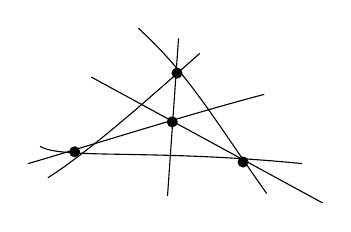
\begin{tikzpicture}[x=.010cm,y=-.010cm]
\draw (25,195) .. controls (80,160) and (157,91) .. (218,37);
\draw (0,177) .. controls (82,153) and (198,116) .. (300,89);
\draw (15,155) .. controls (42,172) and (155,158) .. (348,177);
\draw (80,67) -- (374,227);
\draw (140,5) .. controls (205,65) and (231,113) .. (303,215);
\draw (191,18) -- (177,218);
\foreach \x/\y in {59/162,183/124,189/62,273/175}{\fill (\x,\y) circle[radius=2pt];}
\end{tikzpicture}}

\margin{$6+3=9$ sommets}
$\mathrm{IV}_{7})$ Arrangement d'un quadrilatère et de ses trois diagonales
\figure{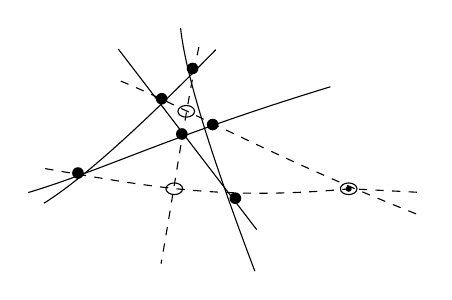
\begin{tikzpicture}[x=.008cm,y=-.008cm]
\draw (25,255) .. controls (87,216) and (181,131) .. (298,11);
\draw (0,238) .. controls (120,202) and (224,148) .. (480,70);
\draw (143,10) -- (363,297);
\draw (242,-23) .. controls (248,30) and (270,125) .. (360,363);
\draw[dashed] (147,61) .. controls (250,103) and (386,181) .. (624,275);
\draw[dashed] (27,200) .. controls (196,229) and (307,251) .. (511,232) -- (627,238);
\draw[dashed] (271,7) .. controls (250,106) and (233,226) .. (211,351);
\foreach \x/\y in {79/207,212/89,261/41,244/145,293/130,329/247}{\fill (\x,\y) circle[radius=2.1pt];}
\foreach \x/\y in {251/109,232/232,509/232}{\draw (\x,\y) ellipse[x radius=3pt,y radius=2.1pt];}
\fill (509,232) circle[radius=1.1pt];
\end{tikzpicture}}

\uline{NB} $\mathrm{III}_{6}$ et $\mathrm{IV}_{7}$ sont \inserted{avec $\mathrm I_{2,2}$ (\unsure{quadri avec|quadr. avec|quadrilatère avec} $1$ diagonale) et $\mathrm I_N$ $(N\geq5)$} les \deleted{configurations} \inserted{\unsure{arrangmts}} avec $N\geq5$ qui ne contiennent pas l'arrangement $\mathrm I'_{3,2}$ ni $\mathrm{II}_5$. Tout \unsure{arrangmt|arrangement} sans bigone, \deleted{contient types et \unsure{qui n'est}} est soit du type $\mathrm{II}_4$, soit contient un des types $\boxed{\mathrm I'_{32},\mathrm{II}_5,\mathrm{III}_6}$ (et s'il ne contient $\mathrm I'_{3,2}$ ni $\mathrm{II}_5$, c'est un type $\mathrm{III}_6$ ou $\mathrm{IV}_7$). Ces trois types \deleted{sont} ``latticiels''\,; i.e. dans le cas 2-dimensionnel, les \unsure{facettes|faces} fermées forment un lattice : \deleted{\unsure{deux}} l'intersection de deux faces fermées non vides est une facette.
% archive sheet number: 24
\scanpage{26}
\mspage{2}
\unsure{hier} auftauchenden Erinnerungen, als auch spätere Perioden meines Lebens \inserted{betreffend}, ohne etwa erst zu warten, bis sie ``dran'' sind. Von grösster Bedeutung bleibt jedenfalls die völlige \unsure{Spontaneität|Spontanëität} der Untersuchung.

Doch könnte ich, im selben Geist der Spontaneität, von \unsure{einem|einer} beliebigen Periode meines Lebens ausgehen, eventuell an Hand von einem reichhaltigen Material wie etwa der Briefwechsel mit Hanka seit 1942. Das wär wohl ein reichhaltiger Ausgangspunkt, wo ein \unsure{wichti}

wiederum das Verhältnis mit \illegible{1} bis zu ihrem Tod, das ich bisher noch nie näher \unsure{betrach|betrachtet} habe. Sollte ich mich \unsure{zue|zuerst} mit diesem ``Stoff'' befassen wäre das eine Art \unsure{Scharn|Scharnier} zwischen der Arbeit der \unsure{l|letzten} sieben Monate, und der, \unsure{d|die} mir bevorsteht. Es könnte einen ``\unsure{Ariane-faden|Arianenfaden}'' \unsure{daraus|davon} \unsure{er|a} weiter zurück in meine \unsure{Ki|Kind}heit -- oder weiter zuvor in Leben als Erwachsener.

Doch bevor ich mich \unsure{einge|eingehend} mit irgend einer Periode \unsure{ode|oder} einer Frage bez. meines Lebens
% archive sheet number: 25
\scanpage{27}
\uline{Cas latticiel} : l'intersection de deux facettes fermées est vide, ou une facette fermée.

\uline{Prop.} Pour qu'on soit dans le cas latticiel il f. et s. que a) Pas de ps. droite ! bigonale, et b) pas du type $\mathrm{II}_{4}$

\uline{Proposition} Soit \inserted{$\unsure{\mathcal X|X}$} un arrgt $\overset{\unsure{?}}{2}$-dim de $N$ ps. droites \inserted{$(D_i)_{i\in I}$}, et considérons une \inserted{$(N+1)^{\text{ième}}$} ps. droite $D$ qui ne soit pas bigonale, \inserted{d'où $\mathcal X'$.} Soit $S$ l'ens des sommets sur $D$ \inserted{de $\mathcal X'$}, i.e. l'ens des intersections de $D$ avec les $D_i$ $(i\in I)$. \deleted{Pour tt $s\in S$, soit $\tilde{s}$ \unsure{la facette} de facettes, \unsure{sur $D_i$|pour $(D_i)$}} Pour que \deleted{$s$ et $s'$,} $s,s'\in S$ soient adjacents sur $D$, il f et s. qu'il existe une face fermée $f$ de $\mathcal X$ qui contienne $s$ et $s'$ -- cette face est alors \unsure{uniquemt|unique} déterminée, et $D\cap f$ est un segment joignant $s$ \unsure{à|,} $s'$, tel que $T\cap f=\{s,s'\}$, c'est aussi l'\inserted{unique} arête sur $D$ joignant $s$ et $s'$ \deleted{\unsure{\}}}.
\figure{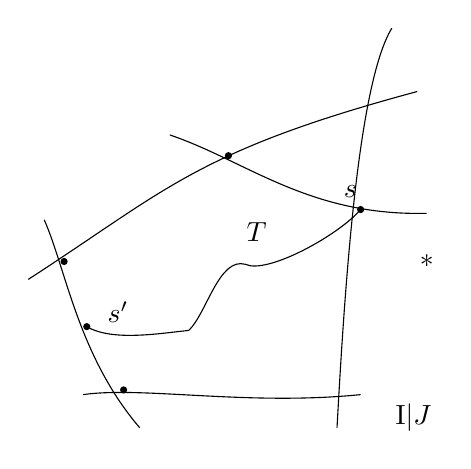
\begin{tikzpicture}[x=.012cm,y=-.012cm]
\draw (5,274) .. controls (152,179) and (183,138) .. (417,75);
\draw (155,121) .. controls (237,149) and (302,207) .. (427,204);
\draw (22,211) .. controls (45,263) and (58,355) .. (123,431);
\draw (63,396) .. controls (126,387) and (237,408) .. (357,396);
\draw (390,8) .. controls (354,67) and (340,284) .. (332,431);
\draw (67,324) .. controls (94,340) and (145,331) .. (175,328) .. controls (194,310) and (207,250) .. (235,258) .. controls (258,269) and (334,227) .. (357,200);
\foreach \x/\y in {67/324,357/200,43/255,217/143,106/391}{\fill (\x,\y) circle[radius=1.3pt];}
\node at (100,309) {$s'$};\node at (346,181) {$s$};\node at (247,224) {$T$};
\node at (413,420) {$\unsure{\mathrm I|J}$};\node at (427,255) {$\unsure{*}$};
\end{tikzpicture}}

\margin{$\mathrm{II}_4\quad\mathrm{II}_5\quad\mathrm{II}_{\unsure{3,2|3,1}},\quad\mathrm{III}_6$}
\deleted{\uline{Lemme} Pour un \unsure{arrangt|arrangement} 1-dim. de $N$ ps. droites sans bigone \inserted{avec $N\geq5$}, on peut trouver \unsure{un arr.} $\mathrm{II}_4$, et une ps. droite $D'$ \unsure{faisant avec celui ci} dans l'un des arrangmts $\mathrm{II}_5,\mathrm{II}_{3,2}$ ou $\mathrm{III}_6$. Quand ensuite on rajoute des ps. droites, elles ne sont jamais bigonales}
% archive sheet number: 26
\scanpage{28}
% letterhead
U N I V E R S I T E\\
DES SCIENCES ET TECHNIQUES\\
\uline{DU LANGUEDOC}

Montpellier, le 13 mai 1981\\
\uline{Service de la Scolarité}\\
Diffusion : Liste A\\
n\textsuperscript{o} 2724\\
AM/MD

\uline{AVIS DE SOUTENANCE D'UNE THESE DE DOCTEUR-INGENIEUR}

PHYSIOLOGIE DE LA NUTRITION DES VEGETAUX

% printed form
\uline{Nom et prénom du candidat} : THIBAUD Jean Baptiste

\uline{Titre de la thèse} : Mécanisme de l'absorption du nitrate par la racine de maïs.

\uline{Date et lieu de soutenance prévus} : 22 mai 1981 à 14 heures, salle de cours n\textsuperscript{o} 7 - U.S.T.L.

\uline{Nom du directeur de thèse} : Monsieur Claude GRIGNON

\uline{Désignation du laboratoire où la thèse est préparée} : Laboratoire de biochimie et physiologie végétale - Centre de recherches agronomiques du Midi 34060 MONTPELLIER CEDEX.

\uline{Résumé de l'ouvrage} : Le mémoire (81 p.) est introduit par une analyse historique dégageant les données acquises sur le problème de l'absorption du nitrate par les végétaux. Le chapitre suivant présente les méthodes, en particulier la réalisation d'un poste d'électrophysiologie. Quatre chapitres de résultats décrivent respectivement le caractère inductible du transporteur de nitrate, les relations avec les échanges de protons, les propriétés stoechiométriques du système, et ses relations avec la pompe à protons de la membrane plasmique. Le chapitre final de discussion présente une analyse critique du modèle retenu (échange 2 nitrate - 1 hydroxyle), examine ses contraintes énergétiques, et propose des directions de recherche. La liste bibliographique comprend 117 références.

\uline{Durée approximative des recherches ayant abouti à la thèse} : 3 ans

\uline{Composition du jury} : M. C. GRIGNON\\
M. J. GUERN\\
M. \unsure{W.|O.} ULLRICH\\
Mme N. PARIS\\
M. JACOB J.L.

P. Le Secrétaire Général,\\
L'Attachée d'Administration Universitaire,\\
\handwritten{\uline{\unsure{Gentil|A. Gentil}}}\\
\uline{A. GENTIL}
% archive sheet number: 27
\scanpage{29}
\uline{Lemme} Soit $\deleted{\unsure{\mathcal X|X}}K$ un arrangt 1-dimensionnel de \inserted{$N$} ps. droites, sans ps. droites bigonales, avec $N\geq5$. Alors on peut ordonner ces $D_1\ldots D_N$, de telle façon que, si $K_i$ désigne l'\unsure{arrangt|arrangement} défini par $D_1\ldots D_i$, alors, pour

$1^\circ)$ $D_1$ -- $D_4$ de type $\mathrm{II}_4$ \deleted{\unsure{ou}} (\deleted{resp.} $D_1$ -- $D_6$ type $\mathrm{III}_6$)

$2^\circ)$ Pour $i\geq5$ \inserted{(resp. $i\geq7$)}, $D_i$ non bigonal dans $K_i$. \deleted{(resp. pour $i\geq7$, $D_i$ \unsure{non}} (NB Dans le cas \unsure{respé|resp.|inverse}, \deleted{\unsure{c'est}} $2^\circ)$ est automatique. \unsure{\}} \deleted{\unsure{NPS que|UPS que}} Dans le \deleted{$K_5$} cas non respé, on peut supposer que $K_5$ est du type $\mathrm{II}_5$, ou du type $\mathrm{II}_{3,2}$, et que les autres types \inserted{$K_i$ $(i\geq6)$} sont $\mathrm{II}_{pq}$, et dans le cas $\mathrm{III}_6$ on peut supposer que $K$ lui-même est $\mathrm{III}_6$, ou $\mathrm{IV}_7$. Pour lemme plus précis,

% slanted
\margin{cas mutuellement exclusifs}
\[\left\{\begin{aligned}
&\text{Ou bien }\exists\, K_5\text{ du type }\mathrm{II}_5\\
&\text{Ou bien }\exists\, K_5\text{ du type }\mathrm{II}_{32},\\
&\text{Ou bien }\deleted{\exists}K\simeq\mathrm{III}_6\text{ ou }\mathrm{IV}_7,
\end{aligned}\right.\]
\margin{-- et quand on continue à rajouter des ps droites $1:1$, c'est pas des bigones}
\margin{et $K$ de type $\mathrm{II}_{pq}$ et alors, quand on rajoute ps-droite, jamais bigonale}
\margin{donc $\exists\,K_6\simeq\mathrm{III}_6$, et \deleted{\unsure{D'}} dans le cas $\mathrm{III}_7$, si on rajoute une ps. droite, elle n'est pas bigonale}

Les pts de départ sont \unsure{de} \deleted{\unsure{telle}} \unsure{façons} $\mathrm{II}_4$ ou $\mathrm{III}_6$.
\figure{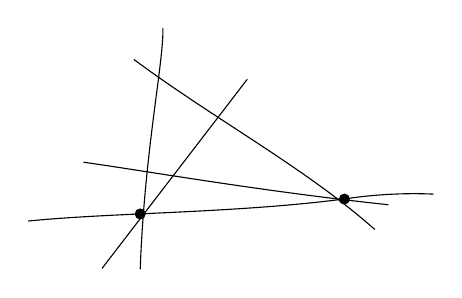
\begin{tikzpicture}[x=.009cm,y=-.009cm]
\draw (2,277) .. controls (120,265) and (293,266) .. (447,246) .. controls (486,240) and (530,237) .. (574,239);
\draw (192,5) .. controls (193,54) and (166,179) .. (160,345);
\draw (106,344) -- (311,77);
\draw (151,49) .. controls (264,133) and (393,202) .. (491,289);
\draw (80,194) .. controls (172,207) and (331,235) .. (510,254);
\fill (160,267) circle[radius=2pt];\fill (448,246) circle[radius=2pt];
\end{tikzpicture}}
% archive sheet number: 28
\scanpage{30}
\mspage{2}
\unsure{hier} auftauchenden Erinnerungen, als auch spätere Perioden meines Lebens \inserted{betreffend}, ohne etwa erst zu warten, bis sie ``dran'' sind. Von grösster Bedeutung bleibt jedenfalls die völlige \unsure{Spontaneität|Spontanëität} der Untersuchung.

Doch könnte ich, im selben Geist der Spontaneität, von \unsure{einem|einer} beliebigen Periode meines Lebens ausgehen, eventuell an Hand von einem reichhaltigen Material wie etwa der Briefwechsel mit Hanka seit 1942. Das wär wohl ein reichhaltiger Ausgangspunkt, wo ein \unsure{wichti}

wiederum das Verhältnis mit \unsure{Hank|Hanka} bis zu ihrem Tod, das ich ja bisher noch nie näher \unsure{betrachte|betrachtet} habe. Sollte ich mich zuerst mit diesem ``Stoff'' befassen, so wäre das eine Art Scharnier zwischen der Arbeit der \unsure{letzt|letzten} sieben Monate, und der, die mir bevorsteht. Es könnte \unsure{sic|sich} einen ``\unsure{Ariane-faden|Arianenfaden}'' \unsure{daraus|davon} \unsure{ergeb|ergeben} weiter zurück in meine Kindheit -- oder weiter zuvor in \unsure{me|mein} Leben als Erwachsener.

Doch bevor ich mich \unsure{eingehen|eingehend} mit irgend einer Periode oder einer Frage bez. meines Lebens \unsure{au}
% archive sheet number: 29
\scanpage{32}
\mspage{1}
I) Arrangements de $3$ pseudo-droites

1) Cube combinatoire (de dim 3). La donnée équivaut à celle d'une famille $(\Phi_i)_{i\in I}$ de trois ens à deux éléments ($\operatorname{card} I=3$, $\operatorname{card}\Phi_i=2\quad\forall i\in I$)
\diagram{(1)\qquad
\begin{tikzcd}[ampersand replacement=\&,column sep=large,row sep=small]
\Phi=\coprod\limits_{i\in I}\Phi_i \arrow[d] \& \text{card }6\\
I \& \text{card }3
\end{tikzcd}}

Les éléments de $\Phi$ s'identifient aux faces du cube, ceux de $I$ aux paires de faces opposées. Les facettes du cube s'identifient aux \uline{sections partielles} de $\Phi$ sur \inserted{des parties $\ne\varnothing$ de} $I$, avec la relation d'incidence correspondant à la relation \uline{opposée} à celle du prolongement de sections partielles, i.e. de l'inclusion des parties correspondantes de $\Phi$ (parties $A\subset\Phi$ non vides, telles que l'appl. induite $A\to I$ soit injective).
\[
\begin{aligned}
 C_2&\simeq\Phi\simeq\mathfrak P_1(\Phi)\\
 C_1&\simeq\{A\in\mathfrak P_2(\Phi)\mid A\to I\text{ injectif}\}\\
 C_0&\simeq\{A\in\mathfrak P_3(\Phi)\mid A\to I\text{ injectif}\ (\text{donc bij.})\}
\end{aligned}\tag*{(2)}
\]
On a \unsure{une|un} automorphisme \inserted{(involutif)} canonique $\underline a$ de (1) induisant l'identité dans $I$ et la transposition dans chacun des $\Phi_i$, qui induit un autom. \inserted{(central)}, encore noté $\underline a$, du cube (2), lequel est l'antipodisme.

Si on prend le polyèdre opposé au cube, on trouve l'octaèdre donné par
\[
\left\{\begin{aligned}
 O_0&=C_2\simeq\Phi\simeq\mathfrak P_1(\Phi)\\
 O_1&=C_1\simeq\{A\in\mathfrak P_2(\Phi)\mid A\hookrightarrow I\}\\
 O_2&=C_0\simeq\{A\in\mathfrak P_3(\Phi)\mid A\unsure{\hookrightarrow|\lhook\joinrel\relbar} I\}
\end{aligned}\right.\tag*{(3)}
\]
avec cette fois-ci la relation \inserted{d'incidence qui est} de prolongement des sections
% archive sheet number: 31
\scanpage{33}
partielles i.e. l'inclusion des parties de $\Phi$.

Passant au quotient par $\underline a$, on trouve le \uline{cube combinatoire \inserted{\uline{gauche} (ou} projectif)} $\widetilde C$, et l'\uline{octaèdre comb. \inserted{\uline{gauche} (ou} projectif)} $\widetilde O$, associé à (1),
\[
\widetilde C_i=C/\{1,\underline a\}\qquad
\widetilde O_i=O/\{1,\underline a\}\tag*{(4)}
\]
(relations d'incidence obtenues en passant au quotient). L'\deleted{\unsure{es}}octaèdre \deleted{projectif} \inserted{gauche} a donc $3$ sommets $6$ arêtes et $4$ faces -- en fait c'est la décomposition du plan projectif réel par un système de trois droites indexées par $I$. (À tout élément $i\in I$, on fait correspondre la ``droite'' correspondant aux deux ``arêtes'' projectives, qui correspondent aux quatre arêtes ordinaires données par $A\in\mathfrak P_2(\Phi)$,
\figure{\begin{tikzpicture}[x=.009cm,y=-.009cm]
\draw (8,233) .. controls (140,246) and (340,213) .. (528,197);
\draw (135,6) .. controls (239,129) and (399,223) .. (550,389);
\draw (49,413) .. controls (101,343) and (207,260) .. (334,62);
\draw (519,191)--(528,197)--(519,201);
\draw (102,341)--(105,349)--(117,340);
\end{tikzpicture}}
$A\overset{\sim}{\longleftrightarrow}I\setminus\{i\}$.

On ne récupère \uline{pas} le cube ou octaèdre ordinaire, à isom canonique près, à partir de la figure \inserted{``gauche''} ``projective'' correspondante, vu que les groupes d'\unsure{inerties|inertie}, dans le cas ordinaire et dans le cas \deleted{projectif}, \inserted{gauche}, ne sont pas isomorphes, plus précisément, $C\mapsto\widetilde C$ resp. $O\vdash\widetilde{C}$
% archive sheet number: 32
\scanpage{34}
\mspage{2}
ne sont pas pleinement fidèles, ni $=$ fidèles, car l'antipodisme $\underline a$ est un autom non trivial de $C,O$ et induit l'autom trivial de $\overline C,\overline O$. Mais on trouve une équiv. de catégories en prenant des cubes comb. \uline{orientés}, des octaèdres combinatoires \uline{orientés}.

\diagram{(5)\quad
\begin{tikzcd}[ampersand replacement=\&,column sep=small]
\text{Cubes comb. orientés}\arrow[r,"\approx"]\arrow[d,"\approx"'] \&
\substack{\text{cubes comb.}\\\text{\deleted{projectifs} \inserted{gauches}}}\arrow[d,"\approx"]\\
\text{octaèdres comb. orientés}\arrow[r,"\approx"] \&
\substack{\text{octaèdres comb.}\\\text{\deleted{projectifs} \inserted{gauches}}}
\end{tikzcd}}

L'ens des orientations du cube, ou de l'octaèdre, donné par (1), est \inserted{donné à isom.} \deleted{\unsure{canonique|canoniquement} \unsure{isomorphe à}} \inserted{près} par
\[
 \operatorname{or}(C)\simeq\operatorname{or}(O)\simeq
 \left(\bigwedge_{i\in I}\Phi_i\right)\wedge\operatorname{or}(I)\tag*{(6)}
\]
où $\operatorname{or}(I)$ \deleted{est} l'ens. des deux ordres circulaires sur $I$ (ou ens des deux ``orientations'' de l'ens fini $I$),
% margin note written sideways
\margin{donc une orientation de $C$, ou $O$, \unsure{revient} à la donnée d'un iso\\
$(6\mathrm{bis})\quad(\bigwedge_{i\in I}\Phi_i)\wedge\operatorname{or}(I)\simeq\mathbb{1}$ ou encore $\bigwedge_{i\in I}\Phi_i\simeq\operatorname{or}(I)$}
À partir de $\widetilde C$ ou $\widetilde O$, on récupère $C$ ou $O$ \deleted{\unsure{avec une orientation}} \inserted{orienté comme le revêtement orienté canonique}.

Soit $i\in I$, d'où ``droite'' $D_i$ de la figure $\widetilde O$. Les deux arêtes de $D_i$ correspondent aux deux bijections $\Phi_j\simeq\Phi_k$ (où $I=\{i,j,h\}$), ou intrinsèquement, aux éléments de
\[
 A_i=\mathop{\deleted{\prod}\bigwedge}_{\alpha\in I\setminus\{i\}}\Phi_\alpha\tag*{(7)}
\]
\margin{(ens des deux arêtes de $\widetilde O$ portées par $D_i$)}
\deleted{Les orient} \unsure{L'ens|L'un} des deux sommets de $D_i$, d'autre part,
% archive sheet number: 33
\scanpage{35}
est donné par
\[
 S_i\simeq I\setminus\{i\}\tag*{(8)}
\]
\margin{\unsure{ens|un} des \inserted{deux} sommets sur la droite}

L'ens des deux orientations de $D_i$ considéré comme support d'un bigône) est donc
\[
 \Omega_i\simeq S_i\wedge A_i\simeq
 \underbrace{(I\setminus\{i\})\wedge
 \underbrace{\bigwedge_{\alpha\in I\setminus\{i\}}\Phi_\alpha}_{\Phi_i\wedge\operatorname{or}(I)}}
 _{\substack{\Phi_i\wedge\bigwedge_{\alpha\in I\setminus\{i\}}(I\setminus\{\alpha\})\\\text{canoniquement}}}\tag*{(9)}
\]
\margin{à cause de (6bis)}

Notons que
\[
\begin{aligned}
 \underbrace{\bigwedge_{i\in I} A_i}_{\shortparallel}&\simeq\mathbb{1}\\
 \bigwedge_{\substack{\alpha,i\in I\\\alpha\ne i}}\Phi_\alpha
 &=\bigwedge_{\alpha\in I}\Phi_\alpha^2\simeq\mathbb{1}
\end{aligned}\tag*{(10)}
\]
d'où
\[
 \bigwedge_{i\in I}\Omega_i\overset{\varphi}{\simeq}
 \bigwedge_{i\in I}S_i
 \left[\simeq\bigwedge_{i\in I}(I\setminus\{i\})
 \underset{\substack{\text{isom can.}\\\text{évident associé}\\\text{à l'ens. à 3}\\\text{éléments }I}}{\overset{\sim}{\leftarrow}}
 \operatorname{or}(I)\right]\tag*{(11)}
\]

\uline{NB} \deleted{Quand} on part d'une famille \deleted{\unsure{de|i.e.}} de trois bigônes $(S_i,A_i)_{i\in I}$, la donnée d'un isom (10) équivaut à celle d'un isom $\varphi\unsure{\}|)}$ (11) (qui, pour $S_i=I\setminus\{i\}\quad\forall i\in I\}$, se réduit à un isom
\[
 \mathop{\deleted{\unsure{\pi}}\bigwedge}\limits_{i\in I}^{\unsure{i'}}\Omega_i\simeq\operatorname{or}(I)\tag*{(11 bis)}
\]
ou encore à un isom
\[
 \left(\bigwedge_{i\in I}^{\unsure{\epsilon|{\,}'}}\Omega_i\right)\wedge\operatorname{or}(I)\simeq\mathbb{1}\tag*{(12)}
\]
% archive sheet number: 34
\scanpage{36}
\mspage{3}
qu'on peut interpréter aussi de la façon suivante : La famille \inserted{$(\Omega_i)_{i\in I}$} des trois ensembles $\Omega_i$ à deux éléments définit un cube -- et on a une orientation de ce cube.

\uline{NB} Les $\Omega_i$ et $\Phi_i$ se déterminent mutuellement par
\[
\left\{\begin{aligned}
 \Omega_i&\simeq\Phi_i\wedge\bigwedge_{\alpha\in I\setminus\{i\}}(I\setminus\{\alpha\})\\
 \Phi_i&\simeq\Omega_i\wedge\bigwedge_{\alpha\in I\setminus\{i\}}(I-\{\alpha\})
\end{aligned}\right.\tag*{(13)}
\]
% slanted
\margin{\unsure{itou pour|idem pour} $\Omega_i$, $\Phi_i$ \deleted{$=$} \inserted{et} $A_i$, puisque
$\begin{aligned}
 A_i&\simeq\deleted{\unsure{\Omega_i\wedge|\bigwedge}}\,(I\setminus\{i\})\deleted{\unsure{S_i}}\\
 &\simeq\Phi_i\wedge\bigwedge_{\alpha\in I}(I-\alpha)\\
 &\simeq\Phi_i\wedge\operatorname{or}(I)
 \end{aligned}$\\ cf (9))}
qui donnent des $\mathrm{isom}^{\mathrm s}$ canoniques
\[
\left\{\begin{aligned}
 \bigwedge_{i\in I}\Omega_i&\simeq\bigwedge_{i\in I}\Phi_i\\
 \text{et}\qquad
 \underbrace{\left(\bigwedge_{i\in I}\Omega_i\right)\wedge\operatorname{or}\,I}
 _{\substack{\text{orientations \unsure{de|avec} l'}\\\text{\unsure{oct.|oct} comb. défini}\\\text{par }(\Omega_i)_{i\in I}}}
 &\simeq
 \underbrace{\left(\bigwedge_{i\in I}\Phi_i\right)\wedge\operatorname{or}\,I}
 _{\substack{\text{orientations de l'oct.}\\\text{comb. défini par}\\(\Phi_i)_{i\in I}.}}
\end{aligned}\right.\tag*{(14)}
\]

En résumé

\uline{Proposition} Considérons la carte combinatoire $\unsure{\mathcal C|\mathscr C}$ (avec trois sommets, six arêtes, quatre faces qui sont des triangles) correspondant à un ``arrangement (combinatoire) de \deleted{quatre} \inserted{trois} ps-droites \inserted{$D_i$ $(i\in I)$} du plan projectif''. Soit $K$ son
% slanted
\margin{octaèdre gauche}
% archive sheet number: 35
\scanpage{37}
squelette de dim 1'' (1-complexe combinatoire, muni du système des trois \deleted{ps.} sous 1-complexes $D_i$. \deleted{On a} Donc $K$ est la réunion des sous\deleted{\unsure{-}} 1-complexes $D_i$, qui sont des bigones, \inserted{chacun} définis par des ens \inserted{à deux él.} de sommets \inserted{$S_i$} et d'arêtes \inserted{$A_i$} \deleted{donnés} \deleted{par} \inserted{avec}
\[
 \deleted{\{S_i\simeq I\setminus\{i\},\ A_i}
\]
\[
 S_i\simeq I-\{i\}
\]
(NB. \deleted{\unsure{Car}} l'ens des sommets de $K$ (i.e. de $\unsure{\mathcal C|C}$) est en corr. biun. avec $I$, en associant à chaque $i\in I$ l'unique sommet qui n'est pas dans $D_i$). Soit
\[
 \Omega_i=S_i\wedge A_i=(I-\{i\})\wedge A_i
\]
l'ens des orientations du bigône $D_i$, i.e. de la ps. droite $\deleted{\unsure{A}}D_i$. Soit
\[
\begin{aligned}
 \Phi_i&=\Omega_i\wedge\bigwedge_{\alpha\in I\setminus\{i\}}(I\setminus\{\alpha\})\\
 &\simeq A_i\wedge\deleted{\unsure{(}}\bigwedge_{\alpha\in I}(I\setminus\{\alpha\})
\end{aligned}
\]
de sorte que l'on a des isom canoniques
\[
 \bigwedge_{i\in I}\Omega_i\simeq\bigwedge_{i\in I}\Phi_i
 \simeq\left(\bigwedge_{i\in I}A_i\right)\wedge
 \underbrace{\bigwedge_{\alpha\in I}(I\setminus\{\alpha\})}_{\operatorname{or} I}\tag*{(15)}
\]
les ens $S_i,\deleted{\unsure{D}}A_i,\Omega_i,\Phi_i$ $(i\in I)$ et les isom
% archive sheet number: 36
\scanpage{38}
\mspage{4}
(15) étant définis donc directement en termes du 1-complexe \inserted{comb.} $K$ et de la donnée des trois ps. droites $D_i\subset K$ dans $K$. On peut réécrire (15) comme un syst. d'iso
\[
 \underbrace{\left(\bigwedge_{i\in I}\Omega_i\right)\wedge\operatorname{or}(I)}
 _{\substack{\text{or. de l'oct.}\\\text{défini par}\\(\Omega_i)_{i\in I}}}
 \simeq
 \underbrace{\left(\bigwedge_{i\in I}\Phi_i\right)\wedge\operatorname{or}(I)}
 _{\substack{\text{or. de l'oct.}\\\text{défini par}\\(\Phi_i)_{i\in I}}}
 \simeq\bigwedge_{i\in I}A_i\tag*{(15 bis)}
\]
Ceci posé, il y a, \deleted{une iso. can. entre} \inserted{du fait que} \uline{$K$ provient de la carte} $C$, \uline{une} \deleted{\unsure{iso}} \inserted{\uline{trivialisation}} \uline{can.} \uline{des} $\mathbb Z/2\mathbb Z$-\uline{torseurs} (15 bis). De façon précise, le foncteur
\diagram{(16)\quad
\begin{tikzcd}[ampersand replacement=\&,column sep=small]
\text{(oct. gauches)}\arrow[r]\&\substack{
\overbrace{\text{graphes octaédraux gauches}}^{\text{gr. oct. gauches}^{+}}\\
\left\{\begin{gathered}
\text{munis d'une trivialisation}\\
\bigwedge_{i\in I} A_i\simeq\mathbb{1}\quad\text{(où }I\text{ est l'ens}\\
\text{des \inserted{3} sommets, et }A_i\text{ est l'}\\
\text{ens des \inserted{2} arêtes qui ne passent}\\
\text{pas par le sommet }i
\end{gathered}\right.}
\end{tikzcd}}
\margin{on appellera cette structure suppl. une \uline{orientation} du gr. octaédral gauche}
est une \uline{équivalence} de catégories

On peut résumer les relations entre octaèdres et graphes octaédraux gauches ou ordinaires, orientés ou non, dans le diagramme de foncteurs suivant (entre groupoïdes connexes)
\diagram{(17)\quad
\begin{tikzcd}[ampersand replacement=\&,column sep=small,row sep=small]
\text{oct}^{+}\arrow[rr,"\approx"]\arrow[dr,"\approx"]\arrow[dd,hook] \& \& \text{oct. gauches}\arrow[dr,"\approx"]\arrow[dd,"\parallel" description] \& \\
\& \text{gr. oct.}^{+}\arrow[rr,"\approx",crossing over]\arrow[dd,hook] \& \& \text{gr oct. gauches}^{+}\arrow[dd,hook]\\
\text{oct.}\arrow[rr]\arrow[dr,"\approx"] \& \& \text{oct. gauche}\arrow[dr,""] \& \\
\& \text{gr. oct.}\arrow[rr,"\approx"] \& \& \text{gr. oct. gauche}
\end{tikzcd}}, 
% archive sheet number: 37
